\documentclass{article}
\usepackage[margin=1in]{geometry}
\usepackage{forest}
\usepackage{listings}
\usepackage{amsmath}
\usepackage{color}
\usepackage{multicol}
\usepackage[colorlinks = true,
            linkcolor = blue,
            urlcolor  = blue,
            citecolor = blue,
            anchorcolor = blue]{hyperref}

\newcommand{\MYhref}[3][blue]{\href{#2}{\color{#1}{#3}}}%

\definecolor{dkgreen}{rgb}{0,0.6,0}
\definecolor{gray}{rgb}{0.5,0.5,0.5}
\definecolor{mauve}{rgb}{0.58,0,0.82}

\lstset{frame=tb,
  language=Java,
  aboveskip=3mm,
  belowskip=3mm,
  showstringspaces=false,
  columns=flexible,
  basicstyle={\small\ttfamily},
  numbers=none,
  numberstyle=\tiny\color{gray},
  keywordstyle=\color{blue},
  commentstyle=\color{dkgreen},
  stringstyle=\color{mauve},
  breaklines=true,
  breakatwhitespace=true,
  tabsize=3
}

\title{CPSC 524 Assignment 1: Divide and Vector Triad Performance}
\author{Rami Pellumbi\thanks{M.S., Statistics \& Data Science}}
\date{\today}

\begin{document}

\maketitle

\newpage 

\section{Introduction}
This assignment investigated the characteristics of the processors on the Grace 
Linux Cluster. First, a program is written to approximate $\pi$ by numerically 
integrating the function 
$$f(x) = \frac{4.0}{1.0 + x^2}$$
from $0$ to $1$. The divide latency is estimated by assuming that floating point 
division cannot be pipelined and assuming that the calculation is dominated by 
the cost of the divide. Next, a program is written to benchmark the performance 
in MFlops of the vector triad kernel. The MFlops are plotted vs. $\log N$, where 
$N$ is the size of the arrays in the vector triad benchmark. The development 
environment was VsCode on MacOS via SSH. The configuration is documented separately 
in \texttt{report/ssh\_vscode\_grace.pdf}.

\section{Project Hierarchy}
The project has the following folder hierarchy:
\begin{multicols}{2}
        \begin{forest}
            for tree={
            font=\ttfamily,
            grow'=0,
            child anchor=west,
            parent anchor=south,
            anchor=west,
            calign=first,
            edge path={
                \noexpand\path [draw, \forestoption{edge}]
                (!u.south west) +(7.5pt,0) |- node[fill,inner sep=1.25pt] {} (.child anchor)\forestoption{edge label};
            },
            before typesetting nodes={
                if n=1
                {insert before={[,phantom]}}
                {}
            },
            fit=band,
            before computing xy={l=15pt},
            }
        [a1
            [build/]
            [common
            [timing.h]
            [timing.c]
            ]
            [part1
            [integrate.c]
            [integrate.h]
            [pi.c]
            ]
            [part2
            [data/]
            [dummy.c]
            [plot.rmd]
            [triad.c]
            [utilities.c]
            [utilities.h]
            ]
            [report/]
            [sbatch-out/]
            [build-run-pi.sh]
            [build-run-triad.sh]
            [Makefile]
        ]
        \end{forest}
    \columnbreak
    \begin{itemize}
        \item \textbf{build}: The \texttt{build} directory is designated for housing the output files generated during the compilation process of both \texttt{part1} and \texttt{part2}. It acts as a repository for these compiled objects, allowing for easier access and management. 
        \item \textbf{common}: The \texttt{common} directory serves as a repository for code that is shared between \texttt{part1} and \texttt{part2}. Specifically, this directory contains the file \texttt{timing.c}, which encapsulates the functionality related to timing measurements. The flag \texttt{-I common} must be in the \texttt{CFLAGS} of the \texttt{Makefile} to ensure this directory is part of the compilation.
        \item \textbf{part1}: The \texttt{part1} directory focuses on the task of numerically estimating the value of \(\pi\). It utilizes a midpoint integration scheme, the details of which are implemented in the \texttt{integrate.c} file. The overall orchestration for estimating \(\pi\) and calculating the latency of division operations is carried out by the \texttt{pi.c} file.
        \item \textbf{part2}: The \texttt{part2} directory houses multiple files, each with distinct responsibilities. The \texttt{dummy.c} file serves the purpose of an opaque function used to ensure our benchmark code runs. The \texttt{triad.c} file is dedicated to performing the vector triad benchmark, an operation that evaluates the memory bandwidth and computational speed for vector operations. Lastly, the \texttt{utilities.c} file contains helper functions for array allocation, initialization with random numbers, and data output to a CSV file for subsequent graphical plotting.
        \item \textbf{report}: The \texttt{report} directory contains the tex files used to write the report and VsCode instruction guide.
        \item \textbf{sbatch-out}: The \texttt{sbatch-out} directory serves as a centralized location for storing all output files generated from code executions on the compute node. The directory's internal folder structure is systematically organized based on the compiler options that led to each individual output file, facilitating easier debugging and performance analysis.
        \item \textbf{build-run-pi.sh}: This is a Bash script specifically crafted to automate the compilation and execution of the code residing in the \texttt{part1} directory. To deploy this script, navigate to the \texttt{a1} directory and execute the command \texttt{sbatch build-run-pi.sh}. This will submit the script to the compute node and subsequently initiate the execution of the Part 1 code.
        \item \textbf{build-run-triad.sh}: Similar to \texttt{build-run-pi.sh}, this Bash script is designed to compile and execute the code for Part 2. Once again, to utilize this script, position yourself in the \texttt{a1} directory and submit the command \texttt{sbatch build-run-triad.sh}. This action will queue the script for execution on the compute node, leading to the running of the Part 2 code.
        \item \textbf{Makefile}: This Makefile has undergone extensive modifications to support the unique build requirements of both \texttt{part1} and \texttt{part2}. It is engineered to handle the appropriate linking of shared libraries and integration of common code components, ensuring a seamless compilation process for both parts. By utilizing this Makefile, the user can effortlessly build and link the code, thereby simplifying the overall build process.
    \end{itemize} 
\end{multicols}

\section{Building and Running the Code}

This section outlines the steps required to build and execute the code for both Part 1 and Part 2 of the project. The provided Bash scripts automate the entire process, making it straightforward to compile and run the code.

\subsection{Automated Building and Execution}
\begin{itemize}
    \item \textbf{Part 1: Numerical Estimation of \(\pi\)} 
    \begin{enumerate}
        \item Navigate to the \texttt{a1} directory if you haven't already.
        \item Run the following command to submit the Part 1 build and execution script: \\
        \texttt{sbatch build-run-pi.sh}
    \end{enumerate}
    This script employs a heavily modified \texttt{Makefile} to handle the compilation and linking of Part 1-specific code.
    
    \item \textbf{Part 2: Vector Triad Benchmark}
    \begin{enumerate}
        \item Make sure you are still in the \texttt{a1} directory.
        \item Execute the following command to submit the Part 2 build and execution script: \\
        \texttt{sbatch build-run-triad.sh}
    \end{enumerate}
    Similar to Part 1, this script utilizes the same modified \texttt{Makefile} to manage the build process for Part 2.
\end{itemize}

\subsection{Post-Build Objects}
Upon successful compilation and linking, a \texttt{build} directory will be generated within the \texttt{a1} root directory. This directory will contain the compiled output files for both parts. Additionally, the executable files for running each part will be situated in the root of the \texttt{a1} directory.

\subsection{Output Files}
The output files generated from running the code will be stored in the root of the \texttt{a1} directory. They are manually moved 
to the \texttt{sbatch-out} directory under the relevant part and compiler options.

\section{Division Performance}
The first benchmark estimates the latency of the divide operation and assesses 
processor performance across different \texttt{icc} compiler options. 
\subsection*{Integration and Timing Setup}
The midpoint integration scheme is done by the function \texttt{integrate\_midpoint\_rule} implemented 
in \texttt{integrate.c} as follows:\footnote{All code shown is roughly similar to the 
submitted code. It is slighlty modified for clear reporting and the official code file 
should be considered as the final submitted solution as it typically is more detailed.}
\begin{lstlisting}
double integrate_midpoint_rule(double start,
                                  double end,
                                  double num_steps,
                                  double (*func)(double))
{
    // width of the interval at each midpoint
    double width_of_interval = 1.0 / num_steps; 
    // initial midpoint is halfway between start and (start + 1/num_steps)
    double current_midpoint = (start + width_of_interval) / 2.0;
    // function value at the midpoint - initialized to the value at inital midpoint
    double current_function_value = func(current_midpoint);

    // initialize the sum value to the first rectangles area
    double sum = current_function_value * width_of_interval;

    // compute each midpoint, function value at that midpoint, and add rectangle area to the sum.
    for (int i = 1; i < num_steps; i++)
    {
        current_midpoint += width_of_interval; // 1 FLOP
        current_function_value = func(current_midpoint);
        sum += current_function_value * width_of_interval; // 2 FLOPS
    }

    return sum;
}
\end{lstlisting}
The function is invoked in \texttt{pi.c} with:
\begin{itemize}
    \item \texttt{start = 0.0}.
    \item \texttt{end = 1.0}.
    \item \texttt{num\_steps = $1000000000$}.
    \item \texttt{func = \texttt{function\_to\_integrate}}.
\end{itemize}
where \texttt{function\_to\_integrate} is 
\begin{lstlisting}
double function_to_integrate(double x)
{
    // 1 divide, 1 add, 1 multiply -> 3 FLOPS
    return 4.0 / (1.0 + x * x);
}
\end{lstlisting}
The results are timed as follows:
\begin{lstlisting}
double start_wc_time = 0.0, end_wc_time = 0.0;
double start_cpu_time = 0.0, end_cpu_time = 0.0;

timing(&start_wc_time, &start_cpu_time);
// Performing 6 FLOPS per iteration, and NUM_STEPS iterations.
double pi = integrate_midpoint_rule(START_X,
                                        END_X,
                                        NUM_STEPS,
                                        function_to_integrate);
timing(&end_wc_time, &end_cpu_time);
\end{lstlisting}
\subsection*{Estimating MFlops and Runtime}
Since we perform 6 floating point operations per iteration of the midpoint integration scheme, 
we perform 6 billion floating point operations between the start of the wall clock time 
and the end of the wall clock time. Thus, we can estimate the runtime in seconds and performance in MFlops by 
\begin{lstlisting}
// runtime
double elapsed_wc_time = end_wc_time - start_wc_time;

// performance in MFlops
double total_number_of_flops = 6.0 * 1e9;
double mega_flops_per_second = total_number_of_flops / elapsed_wc_time / 1.0e6;
\end{lstlisting}
\subsection*{Runtime of Algorithm Across Compiler Options: Performance in MFlops Using One Core of One Compute Node}
The results of the $\pi$ estimate, estimated MFlops, and elapsed wallclock time are shown for the following four compiler options:
\begin{enumerate}
    \item \texttt{-g -O0 -fno-alias -std=c99}
    \begin{lstlisting}
    pi estimate = 3.141593
    elapsed wall clock time = 4.896937
    Estimated MFLOPS = 1225.255732

    real	0m4.901s
    user	0m4.891s
    sys	0m0.002s
    \end{lstlisting}
    \item \texttt{-g -O3 -no-vec -no-simd -fno-alias -std=c99}
    \begin{lstlisting}
    pi estimate = 3.141593
    elapsed wall clock time = 2.655869
    Estimated MFLOPS = 2259.147565
    
    real	0m2.660s
    user	0m2.652s
    sys	0m0.002s
    \end{lstlisting}
    \newpage
    \item \texttt{-g -O3 -fno-alias -std=c99}
    \begin{lstlisting}
    pi estimate = 3.141593
    elapsed wall clock time = 2.655767
    Estimated MFLOPS = 2259.234369
    
    real	0m2.661s
    user	0m2.654s
    sys	0m0.001s
    \end{lstlisting}
    \item \texttt{-g -O3 -xHost -fno-alias -std=c99}
    \begin{lstlisting}
    pi estimate = 3.141593
    elapsed wall clock time = 2.655834
    Estimated MFLOPS = 2259.177175
    
    real	0m2.670s
    user	0m2.653s
    sys	0m0.002s
    \end{lstlisting}
\end{enumerate}
Some notes on what these options mean and the differences in each run:
\begin{itemize}
    \item The compiler optimizations do not impact the accuracy of the algorithm.
    \item All options include \texttt{-g -fno-alias -std=c99} which means we generate 
    debuggin information, disable pointer aliasing, and use the C99 standard, respectively.
    \item The flag \texttt{-O0} disables compilor optimizations while the flag \texttt{-O3} offers aggressive and extensive optimizations.\footnote{\MYhref{https://www.intel.com/content/www/us/en/docs/cpp-compiler/developer-guide-reference/2021-8/o-001.html}{Optimizations Compiler Documentation.}}
    \item The flags \texttt{-no-vec -no-simd} together disable all compiler vectorization.\footnote{\MYhref{https://www.intel.com/content/www/us/en/docs/cpp-compiler/developer-guide-reference/2021-8/simd-qsimd.html}{SIMD Compiler Documentation.}}
    \item The flag \texttt{-xHost} tells the compiler to generate instructions for the highest instruction set available on the compilation host processor. Given the host processor is an Intel(R) Xeon(R) Platinum 8268, using \texttt{-xHost} 
    means the compiler may use AVX-512 instructions, fused multiply add instructions, and bit manipulation.\footnote{\MYhref{https://www.intel.com/content/www/us/en/docs/cpp-compiler/developer-guide-reference/2021-8/xhost-qxhost.html}{xHost Compiler Documentation.} The CPU flags were assessed from running \texttt{lscpu} and inferring what the compiler may do.}
\end{itemize}
Given the flag information and performance results, it can be concluded that:
\begin{itemize}
    \item Options 2, 3, and 4 are very similar. We can reasonably conclude that vectorization is not a component of this algorithm. 
    \item The \texttt{-O0} flag results in very slow execution, illustrating the impact of compiler optimizations.
\end{itemize}
The performance is what I expected for the first and fourth compiler option. Going into the problem, I expected disabling vectorization 
would decrease performance but this was not the case. This makes sense given the lack of vectorization in the program.

\subsection*{Divide Latency Estimate}
Assuming the performance of the $\pi$ calculation is dominated by the cost of the division operations, 
and assuming that division cannot be pipelined, we can estimate the latency of the divide operation by disabling 
all compiler optimization and computing the total number of cycles in our integration scheme divided by the total number of 
steps, e.g.,: 
\begin{lstlisting}
// found via lscpu on the compute node in the "CPU MHz:" row. 
// Assumed all cores run at this frequency.
double cpu_frequency_hertz = 3.5e9;
double total_number_of_cycles = elapsed_wc_time * cpu_frequency_hertz;
double estimated_divide_latency = total_number_of_cycles / num_steps;
\end{lstlisting}
The specific compiler option used was: \texttt{-g -O0 -fno-alia -no-vec -no-simd}. This 
resulted in an estimated divide latency of about 17 cycles. The compiler options do matter in estimating this latency. 
For example, when running option 4 from before, the estimated divide latency is about 9 cycles. When the compiler 
is able to do aggressive optimizations, our assumptions begin to have less validity and the estimation is not as accurate, e.g., 
if multiple divides are being concurrently performed in the optimized version we have to account for that in our latency estimate.


\section{Vector Triad Performance}
The second benchmark measures the performance in MFlops of the vector triad kernel: 
$$
\texttt{a[i]} = \texttt{b[i]} + \texttt{c[i]} * \texttt{d[i]},
$$
where \texttt{a}, \texttt{b}, \texttt{c}, and \texttt{d} are double precision arrays 
of length \texttt{N} initialized with values in $[0, 100]$. The arrays are allocated memory and initialized via the following two helper functions:
\begin{lstlisting}
void *allocate_double_array(size_t num_elements)
{
    // allocate uninitialized memory
    void *array = malloc(num_elements * sizeof(double));

    // exit if allocation failed
    if (array == NULL) exit(1);

    return array;
}

void initialize_array_with_random_numbers(double *array, size_t num_elements)
{
    // for each element in the array, store a random double in [0,100]
    for (size_t i = 0; i < num_elements; ++i)
    {
        array[i] = ((double)rand() / (double)RAND_MAX) * 100.0;
    }
}
\end{lstlisting}

\subsection*{Setting up the Benchmark}
The performance benchmark ensures that the program runs for at least 1 second in duration. 
To ensure the operations in the kernel actually get executed, we insert a conditional call 
to an opaque function \texttt{dummy} residing in \texttt{dummy.c}. The expression in the conditional 
is such that the compiler can not easily determine the result of the conditional statement at compile time. 
The expression of choice is \texttt{a[N >> 1] > 0}, which is always \texttt{false} when $a$ is initialized with positive numbers. 
The benchmark is summarized in the following snippet:
\newpage
\begin{lstlisting}
int number_of_repetitions = 1;
double runtime = 0.0;
while (runtime < 1.0)
{
    // start the timing
    timing(&start_wc_time, &start_cpu_time);
    for (int r = 0; r < number_of_repetitions; ++r)
    {
        for (size_t i = 0; i < num_elements; i++)
        {
            a[i] = b[i] + c[i] * d[i];
        }

        // this if condition is always false when a is initiated with all positive values
        if (a[num_elements >> 1] < 0) dummy(a, b, c, d);
    }
    // end the timing
    timing(&end_wc_time, &end_cpu_time);
    runtime = end_wc_time - start_wc_time;
    number_of_repetitions *= 2;
}
number_of_repetitions /= 2;
\end{lstlisting}
The benchmark itself takes place in \texttt{part2/triad.c} and the script 
takes as input a positive integer \texttt{k}. The length \texttt{N} is then computed as 
$$
\texttt{N} = \texttt{floor}(2.1^k).
$$
The benchmark is run for $k$ in the inclusive range $3...25$. The script \texttt{build-run-triad.sh} has a 
simple for-loop to provide the triad program with each value of $k$:
\begin{lstlisting}
for k in {3..25}
do
  echo "Running with k = $k"
  time ./triad $k
done
\end{lstlisting}
Each call of the program will output the total megaflops per second and number of elements in the arrays to 
\texttt{part2/data/part\_2\_data.csv} via the helper function \texttt{write\_data\_to\_file} located in 
\texttt{part2/utilities.c}. Since each iteration of the vector triad is two floating point operations, we compute the total 
floating point operations to be the number of repetitions times the number of elements in the array times 2 divided by the runtime 
converted to megaflops:
\begin{lstlisting}
double total_mega_flops = 2.0 * (double)N * number_of_repetitions / runtime / 1.0e6;
\end{lstlisting}
Running under the compiler options \texttt{-g -O3 -xHost -fno-alias -std=c99}, we produce the following application output for $k=5, 11, 22$:
\begin{lstlisting}
Running with k = 5

number of array elements: 40
134217728 repetitions performed
elapsed wall clock time = 1.234365
elapsed cpu time = 1.232172
estimated MFLOPS: 8698.738508
real	0m2.476s
user	0m2.464s
sys   0m0.002s

Running with k = 11

number of array elements: 3502
1048576 repetitions performed
elapsed wall clock time = 1.152193
elapsed cpu time = 1.149823
estimated MFLOPS: 6374.128172
real	0m2.306s
user	0m2.295s
sys   0m0.002s

Running with k = 22

number of array elements: 12269432
32 repetitions performed
elapsed wall clock time = 1.239635
elapsed cpu time = 1.235572
estimated MFLOPS: 633.447470
real	0m2.826s
user	0m2.739s
sys   0m0.073s
\end{lstlisting}
In total, 8 jobs were submitted to slurm via \texttt{sbatch}. Each job output the results of megaflop performance vs. \texttt{N} 
in \texttt{part2/data/part\_2\_data.csv} for every \texttt{k} value. The csv file was loading using the \texttt{plot.rmd} file to show the performance in MFlops versus \texttt{log N}.

\subsection*{Assessing Performance vs. Array Size}
Having 8 data points for each value of \texttt{k}, the plot below shows the average 
MFlops versus $\log_2 \texttt{N}$. The red lines are the standard deviation from the mean.

\begin{multicols}{2}
    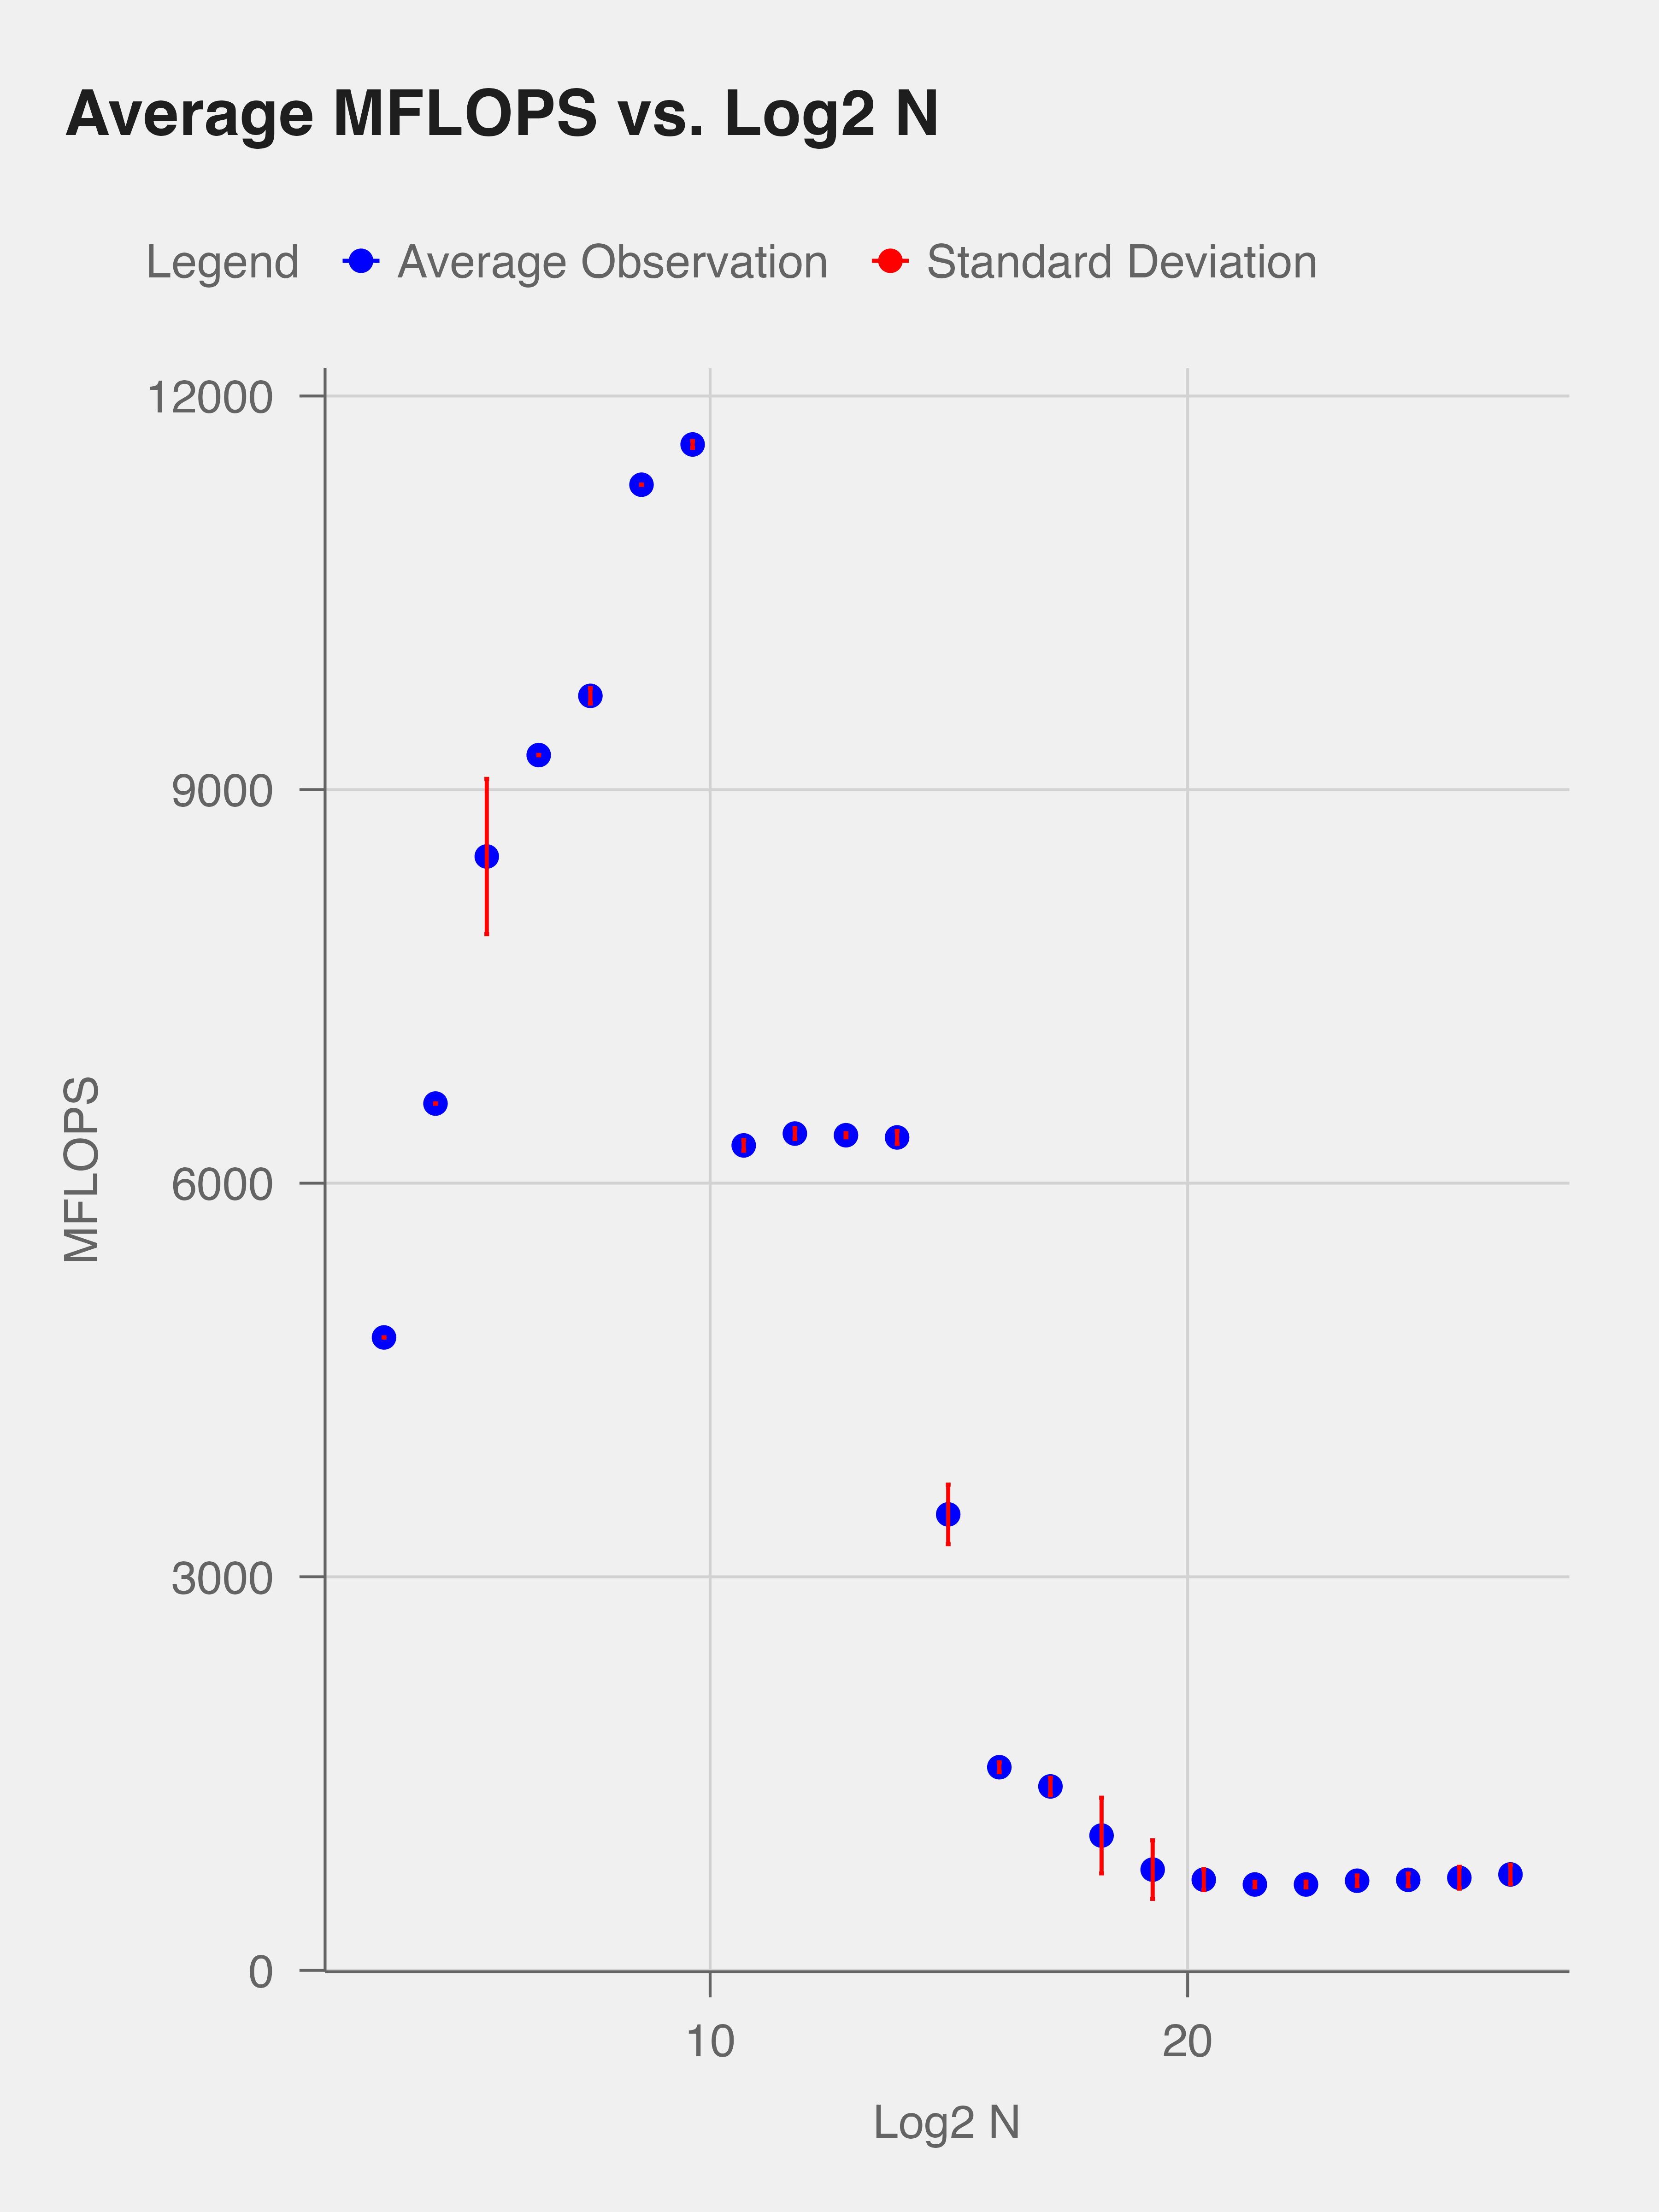
\includegraphics[width=.45\textwidth]{../part2/data/part_2_plot.png}
    \columnbreak
    
    \ 

    \noindent The plot results are quite interesting. First, a bit of processor information. The Intel(R) Xeon(R) Platinum 8268 processor has: 
    \begin{itemize}
        \item 24 $\times$ 32K \texttt{L1d} cache (stores data). This is 8-way set associative with write-back.
        \item 24 $\times$ 32K \texttt{L1i} cache (stores instructions for cores to execute). This is 8-way set associative.
        \item 24 $\times$ 1024K \texttt{L2} cache. This is 16-way set associative with write-back.
        \item 1 $\times$ 36608K \texttt{L3} cache. This is 11-way set associative with write-back. It is shared by every core 
        on the processor.
    \end{itemize}
    Moreover, 
    \begin{itemize}
        \item The \texttt{L2} cache is inclusive.
        \item The \texttt{L3} cache is shared by every core on the chip. 
        \item The \texttt{L3} cache is not inclusive.
    \end{itemize}
\end{multicols}
\newpage
Knowing our cache information, the performance starts to make sense. The benchmark was run on 1 core of a single node and thus 
we have access to 1 of each of the level 1 and 2 caches. 

\end{document}

